\documentclass[12pt,a4paper]{report}
\usepackage[T1]{fontenc}
\usepackage[a4paper,left=1.5in,right=1.25in,top=1.25in,bottom=1.25in,headheight=15pt]{geometry}
\usepackage{mathptmx}
\usepackage{array}
\usepackage{tabularx}
\usepackage[table]{xcolor}
\usepackage{graphicx}
\usepackage{acronym}
\usepackage{enumitem}
\usepackage{setspace}
\usepackage{fancyhdr}
\usepackage{titlesec}
\usepackage{cite}
\usepackage{caption}
\usepackage{hyperref}
\usepackage{xurl}
\usepackage{pdflscape}
\usepackage{pgfgantt}
\usepackage{tikz}
\usetikzlibrary{arrows.meta,positioning}

\graphicspath{{./images/}{./}}
\urlstyle{same}

\hypersetup{
    colorlinks=true,
    linkcolor=black,
    citecolor=black,
    urlcolor=blue,
    breaklinks=true
}

\onehalfspacing
\setlength{\parindent}{0pt}
\setlength{\parskip}{8pt}

\pagestyle{fancy}
\fancyhf{}
\fancyfoot[C]{\thepage}
\renewcommand{\headrulewidth}{0pt}
\renewcommand{\bibname}{References}
\newcolumntype{Y}{>{\raggedright\arraybackslash}X}

\titleformat{\chapter}[display]
{\normalfont\bfseries\Large\centering}
{\chaptername\ \thechapter}{10pt}{\Large}
\titleformat{\section}
{\normalfont\bfseries\large}{\thesection}{1em}{}
\titleformat{\subsection}
{\normalfont\bfseries\normalsize}{\thesubsection}{1em}{}

\newcommand{\studentname}{Bikash Kumar Sah}
\newcommand{\rollnumber}{16}
\newcommand{\programname}{B.Tech in Artificial Intelligence}
\newcommand{\semesterinfo}{IV Year, I Semester}
\newcommand{\submissiondate}{April 6, 2026}

\newcommand{\insertkulogo}{%
    \IfFileExists{images/ku.png}{\includegraphics[scale=0.12]{images/ku.png}}{%
    \IfFileExists{ku.png}{\includegraphics[scale=0.12]{ku.png}}{%
    \IfFileExists{ku_logo.png}{\includegraphics[scale=0.12]{ku_logo.png}}{%
    \IfFileExists{images/ku_logo.png}{\includegraphics[scale=0.12]{images/ku_logo.png}}{%
        \vspace{1.0cm}%
    }}}}%
}

\begin{document}

\begin{titlepage}
    \thispagestyle{empty}
    \begin{center}
        \huge \textbf{Kathmandu University}\\[6pt]
        \Large \textbf{School of Engineering}\\[6pt]
        \Large \textbf{Department of Artificial Intelligence}\\
        \large \textbf{Dulikhel, Kavre}\\[10pt]

        \insertkulogo\par\vspace{8pt}

        \large \textbf{Semester Project Proposal}\\[2pt]
        \large In partial fulfillment of the requirements for\\
        \large \semesterinfo\ of \programname\\[12pt]

        \rule{\textwidth}{0.6pt}\\[6pt]
        \begin{minipage}{0.93\textwidth}
            \centering
            \fontsize{14}{16}\selectfont\textbf{MarketGyan: NEPSE and Financial News Analysis}\\[2pt]
            \fontsize{14}{16}\selectfont\textbf{An Extension of Khabar AI}
        \end{minipage}\\[6pt]
        \rule{\textwidth}{0.6pt}\\[16pt]
        \vspace{0.4cm}

        \begin{tabular}{rl}
            \textbf{Submitted by:} & \studentname \\
            \textbf{Roll Number:} & \rollnumber \\
            \textbf{Submission Date:} & \submissiondate \\
        \end{tabular}

        \vspace{0.6cm}

        \textbf{Submitted to}\\
        Head of Department\\
        Department of Artificial Intelligence
    \end{center}
\end{titlepage}

\pagenumbering{roman}

\chapter*{Abstract}
\addcontentsline{toc}{chapter}{Abstract}
Investors in Nepal rely on sources such as \ac{NEPSE} summaries, financial news portals, and regulatory notices to understand daily market movement. However, these sources are fragmented and difficult to synthesize quickly. This proposal presents \textit{MarketGyan}, an extension of existing \textit{Khabar AI} platform into a Nepal-specific financial-analysis assistant. The proposed system combines automated post-market data collection, a \ac{RAG} layer over financial news and regulatory documents, a fine-tuned multilingual instruction model in the 7B--10B range, and an agent-based workflow for evidence gathering, analysis, and report generation. It will ingest market-close indicators and finance-related articles, store both English and Nepali text for retrieval, process selected \ac{NRB} and \ac{SEBON} PDFs , estimate article- and sector-level sentiment, and generate daily reports and user-facing answers with source support. The use of a stronger model class such as Qwen2.5-7B or Llama 3.1 8B is intended to support multilingual processing, constrained tool use, and more informative event-based explanations. Evaluation will consider sentiment-classification performance, retrieval usefulness, factual grounding, report quality, freshness, and response latency. The expected outcome is a Nepal-specific financial-analysis system and a study of how fine-tuning, retrieval, agents, and automation can be combined effectively.

\tableofcontents
\clearpage

\listoffigures
\addcontentsline{toc}{chapter}{List of Figures}
\clearpage

\chapter*{List of Abbreviations}
\addcontentsline{toc}{chapter}{List of Abbreviations}
\begin{acronym}[QLoRA]
    \acro{AI}{Artificial Intelligence}
    \acro{API}{Application Programming Interface}
    \acro{ETL}{Extract, Transform, Load}
    \acro{F1}{F1-Score}
    \acro{JWT}{JSON Web Token}
    \acro{LLM}{Large Language Model}
    \acro{LoRA}{Low-Rank Adaptation}
    \acro{NEPSE}{Nepal Stock Exchange}
    \acro{NLP}{Natural Language Processing}
    \acro{NRB}{Nepal Rastra Bank}
    \acro{PEFT}{Parameter-Efficient Fine-Tuning}
    \acro{QLoRA}{Quantized Low-Rank Adaptation}
    \acro{RAG}{Retrieval-Augmented Generation}
    \acro{RSS}{Really Simple Syndication}
    \acro{SEBON}{Securities Board of Nepal}
    \acro{UI}{User Interface}
\end{acronym}
\clearpage

\pagenumbering{arabic}

\chapter{Introduction}

\section{Background and Motivation}
Retail investors in Nepal follow the stock market through a combination of \ac{NEPSE} summaries, broker portals, social-media discussion, financial news sites, and regulatory notices. However, the information required to understand a single trading day is highly fragmented. Price movement, turnover, sector changes, and top gainers may come from the exchange or market portals, while the possible reasons for those movements are often scattered across separate articles, interviews, circulars, and monetary-policy announcements. As a result, users must manually connect structured market data with unstructured financial news before forming even a basic interpretation of market sentiment.

This project builds on earlier work on \textit{Khabar AI}, which already includes \ac{RSS} ingestion, semantic search with Qdrant, AI-generated summaries, personalized newsletters, and scheduled jobs. Instead of building a new platform from the beginning, the present work extends that system for finance-specific analysis. This allows the project to focus on domain adaptation, financial retrieval, sentiment analysis, and automated market reporting.

\section{Proposed System}
The proposed system, \textit{MarketGyan}, is designed as an analytical assistant for the Nepali equity market. It will track daily \ac{NEPSE} data, collect local financial news, index the content for semantic retrieval, estimate article- and sector-level sentiment using a fine-tuned domain model, and produce outputs such as:
\begin{itemize}[leftmargin=1.6em]
    \item a daily after-market summary report;
    \item sector-wise sentiment snapshots;
    \item grounded answers to user queries such as ``What news may have affected hydropower stocks today?''; and
    \item scheduled financial newsletters or Telegram-style bulletins.
\end{itemize}

\section{Problem Statement}
The core problem is to develop a Nepal-specific financial-analysis system that can combine structured stock-market indicators with local financial news and regulatory updates. A simple scraping dashboard would not be sufficient for this purpose, while a full trading platform would be outside the intended scope. The proposed work therefore focuses on a research prototype that combines \ac{RAG}, fine-tuning, agent-based reasoning, and automation using the existing Khabar AI codebase.

\section{Objectives}
The project has four objectives:
\begin{enumerate}[leftmargin=1.6em]
    \item extend the existing Khabar AI platform so that it can collect \ac{NEPSE} market data, financial news, and selected regulatory documents for daily analysis;
    \item develop a multilingual retrieval and document-processing pipeline that can handle English articles, Nepali articles, and cleaned OCR text from selected PDFs;
    \item fine-tune a 7B--10B class instruction model for financial sentiment analysis, market explanation, and structured report generation; and
    \item evaluate the proposed system using sentiment, retrieval, grounding, and report-quality measures.
\end{enumerate}

\section{Scope and Feasibility}
The scope is limited to publicly available market data and news. The system will not connect to user brokerage accounts, place trades, provide personalized portfolio management, or issue direct buy or sell recommendations. The focus is analytical assistance rather than investment advice. The project will use a multilingual 7B--10B instruction model so that both English and Nepali source text can be processed during retrieval and analysis. The project remains feasible  because:
\begin{itemize}[leftmargin=1.6em]
    \item Khabar AI already provides the base web app, authentication, scheduler, search stack, and newsletter infrastructure;
    \item \ac{NEPSE} and local financial news are updated daily and can be collected with moderate effort;
    \item most of the new complexity lies in the analysis layer rather than in rebuilding the full application stack; and
    \item the fine-tuning task can be bounded to sentiment, event explanation, and structured report generation rather than large-scale financial forecasting.
\end{itemize}

\chapter{Related Work and Technical Context}

\section{Nepal-Specific NLP and Multilingual Processing}
Work on Nepali NLP remains more limited than work on high-resource languages, but recent studies provide a stronger foundation than was available even a few years ago. Timilsina et al. introduced NepBERTa, a monolingual Nepali language model trained on a large news corpus, and showed that language-specific pre-training improves multiple Nepali NLP tasks \cite{timilsina2022}. Subedi et al. later evaluated large language models for Nepali named-entity recognition and part-of-speech tagging, highlighting both the promise of modern transformer models and the continuing importance of low-resource benchmarks \cite{subedi2024}. Thapa et al. further expanded the available Nepali model landscape by training new encoder and decoder models on a substantially larger monolingual corpus and reporting gains on both understanding and generation tasks \cite{thapa2025}. These studies suggest that Nepali text can now be processed more directly in applied systems, especially when multilingual or Nepali-adapted models are combined with careful fine-tuning.

\section{Financial NLP and Financial LLMs}
Financial text differs from general news because it contains domain-specific terminology, event-driven sentiment, and interpretation that depends on policy, regulation, and sector context. Earlier work such as FinBERT established that domain adaptation improves financial sentiment analysis compared with general-purpose language models \cite{araci2019finbert}. Since 2023, research has shifted toward broader financial LLM ecosystems. Yang et al. presented FinGPT as an open-source financial LLM effort built around financial-data curation and lightweight adaptation \cite{yang2023fingpt}. Lee et al. surveyed the FinLLM literature and summarized major training strategies, benchmark tasks, and persistent risks such as hallucination and weak evaluation \cite{lee2024finllms}. Bhatia et al. introduced FinTral, a multimodal financial LLM family built on Mistral-7B and adapted through domain-specific pre-training and instruction tuning \cite{bhatia2024fintral}. Together, these studies support the use of a moderately sized, finance-adapted model in the proposed system.

\section{Fine-Tuning and Parameter Efficiency}
Fine-tuning is important in the present project because the analyst component should do more than classify generic positive or negative tone. It should learn a domain-specific output format such as \texttt{market direction}, \texttt{affected sector}, \texttt{reason}, and \texttt{confidence}. LoRA enables efficient adaptation by learning low-rank weight updates instead of updating the full parameter set \cite{hu2021lora}, while \ac{QLoRA} makes such experiments more feasible on limited hardware \cite{dettmers2023qlora}. These approaches are especially suitable, where model size and training cost must remain manageable.

\section{Retrieval-Augmented Generation}
\ac{RAG} combines external retrieval with generation so that responses can be grounded in fresh documents instead of static model memory \cite{lewis2020rag}. This is especially relevant in finance because articles, market summaries, and regulatory notices change daily. A model that relies only on fine-tuned weights will quickly become stale. In the proposed system, the retrieval layer will provide current evidence while the fine-tuned model will contribute financial interpretation and answer formatting.

\section{Agent-Based Workflows and Tool Use}
Recent work on LLM agents suggests that stronger instruction models can support more structured planning, tool use, and coordination than earlier systems. ReAct showed that reasoning and acting can be interleaved so that a model can retrieve information and update its decisions during inference \cite{yao2023react}. AutoGen later framed multi-agent interaction as a practical engineering pattern for building applications through coordinated conversations between specialized agents and tools \cite{wu2023autogen}. Guo et al. surveyed LLM-based multi-agent systems and described common designs for role assignment, communication, and task decomposition \cite{guo2024multiagentsurvey}. These studies support the use of a constrained agent-based workflow in the present project, provided that the roles, tools, and output schemas are kept simple and well defined.

\chapter{Methodology}

\section{Leveraging the Existing Khabar AI Platform}
The proposed project directly builds on existing Khabar AI implementation. Several current modules can be reused with limited adaptation:

\begin{table}[htbp]
\centering
\small
\begin{tabularx}{\textwidth}{|p{2.7cm}|Y|Y|}
\hline
\textbf{Existing Khabar AI component} & \textbf{Current role} & \textbf{Planned MarketGyan AI adaptation} \\
\hline
News fetching and scheduler modules & Periodic \ac{RSS} collection and article updates & Collect finance-only feeds and trigger post-market ETL jobs \\
\hline
Embedding and Qdrant services & Multilingual embeddings and semantic search & Index finance articles, \ac{NRB} circulars, and company-related chunks for \ac{RAG} \\
\hline
Email and newsletter services & Automated personalized newsletters & Generate daily market digest emails after \ac{NEPSE} closes \\
\hline
React frontend and Express backend & User interface, authentication, and APIs & Add market dashboard, query interface, report view, and sector filters \\
\hline
Existing AI summary flow & General article summaries & Produce finance-specific news summaries and sector commentary \\
\hline
\end{tabularx}
\caption{How the existing Khabar AI platform will be reused in the proposed project.}
\label{tab:khabar-reuse}
\end{table}

This reuse reduces implementation effort and allows the project to focus on the finance-specific components.

\section{Data Sources}
The project will combine structured market data and unstructured text data. Structured data will include daily \ac{NEPSE} summaries such as index movement, turnover, sector indices, top gainers, top losers, and volume leaders from official or widely used market sources \cite{nepse-official,sharesansar}. Unstructured data will include financial articles and regulatory notices from sources such as Sharesansar, Kathmandu Post Money, Republica business coverage, and text-based \ac{NRB} or \ac{SEBON} notices \cite{nrb-official,kathpost-money}.

\begin{table}[htbp]
\centering
\small
\begin{tabularx}{\textwidth}{|p{2.7cm}|Y|Y|p{2.1cm}|}
\hline
\textbf{Data type} & \textbf{Example fields} & \textbf{Use in system} & \textbf{Collection difficulty} \\
\hline
\ac{NEPSE} market data & Index close, turnover, sector changes, gainers, losers, volume leaders & Daily report generation, sector context, query answering & Low to moderate \\
\hline
Financial news articles & Headlines, article body, source, date, company or sector mentions & Sentiment analysis, \ac{RAG}, summarization, report evidence & Low \\
\hline
\ac{NRB} and \ac{SEBON} documents & Text notices, web circulars, and selected policy documents & Regulatory grounding and event explanation & Moderate to High \\
\hline
Historical labeled dataset & Bullish, bearish, neutral labels with short explanations & Fine-tuning and evaluation & Moderate \\
\hline
\end{tabularx}
\caption{Planned data inputs for MarketGyan AI.}
\label{tab:data}
\end{table}

\section{Data Acquisition Strategy}
The project will use a primary-and-fallback acquisition strategy. For market data, official \ac{NEPSE} pages will be used whenever the required information is available in a stable and machine-readable form. If an official page does not expose a required sector or summary field consistently, a secondary public market portal will be used and the source of each field will be logged. For news articles, \ac{RSS} or article pages will be collected with source metadata, publication date, and link. For regulatory documents, the system will first attempt to collect web text directly; when only PDF documents are available, an OCR step will be applied. This record of source provenance is important because the final reports should cite the evidence used for each explanation.

\section{Document Extraction and Language Handling}
The system will store English and Nepali documents in their original form whenever possible. English articles will be indexed directly. Nepali articles that are already available as machine-readable text will also be stored directly in Qdrant, allowing the multilingual model to reason over the raw text without an intermediate translation step. English summaries may still be generated for reporting and evaluation. For regulatory documents distributed as PDFs, the system will apply OCR to obtain raw text and then pass the extracted text through an \ac{LLM}-assisted cleaning step to correct broken characters, missing spaces, and obvious OCR errors before indexing. The original text, cleaned text, and source link will be stored together for traceability.

\section{Overall System Architecture}
Figure~\ref{fig:architecture} summarizes the proposed system. The design separates data acquisition, storage, retrieval, analysis, and publication so that each layer can be evaluated independently during the semester.

\begin{figure}[htbp]
\centering
\resizebox{\textwidth}{!}{%
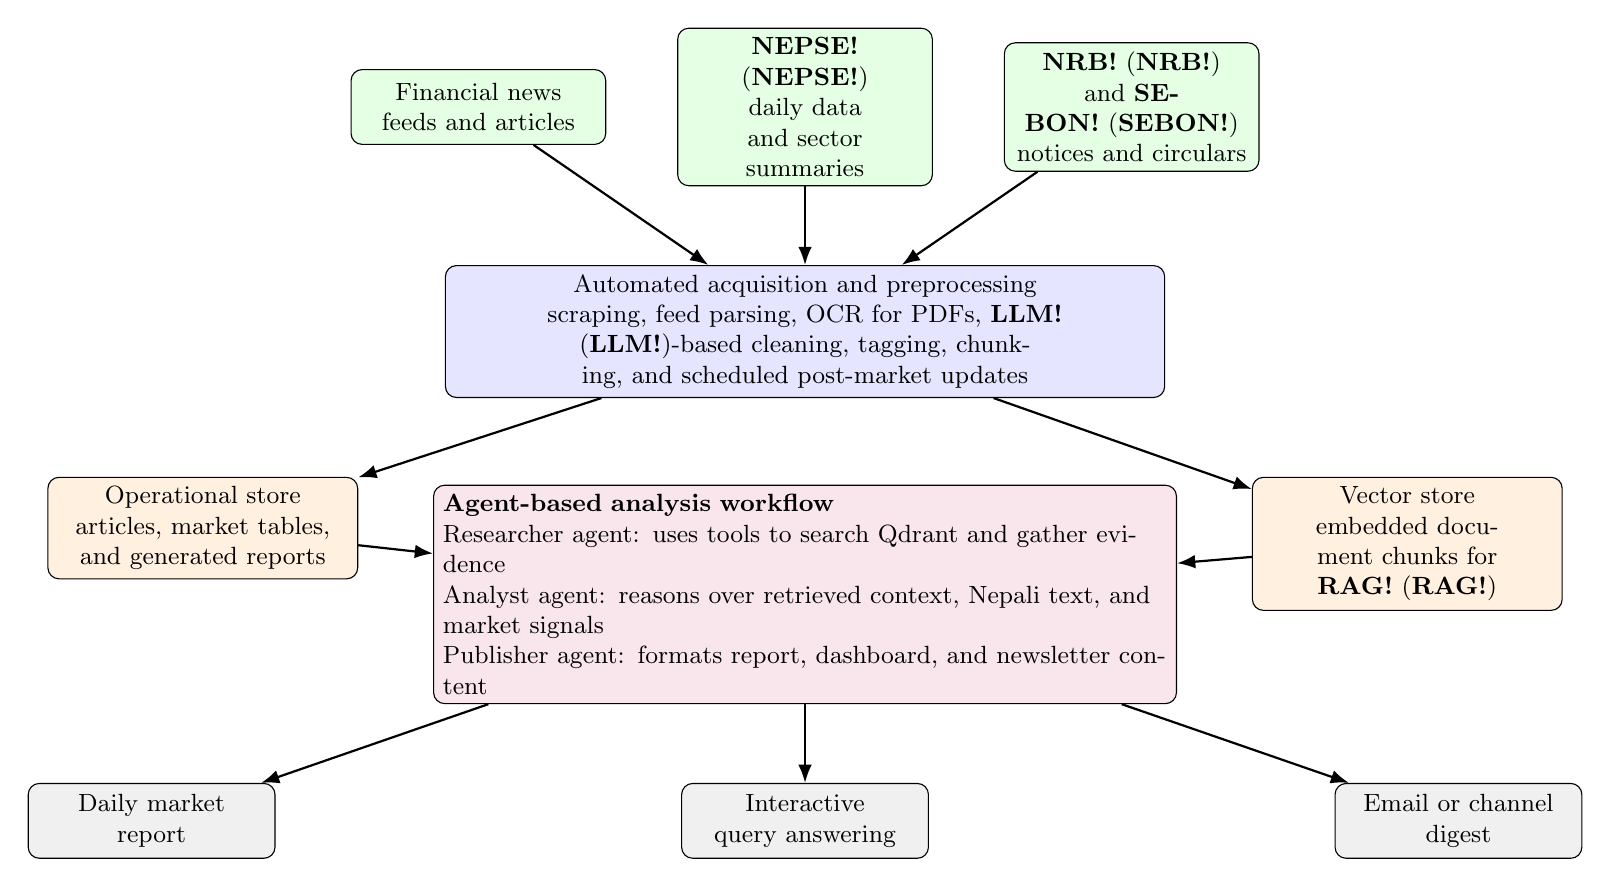
\begin{tikzpicture}[
    >=Latex,
    node distance=0.9cm and 0.9cm,
    every node/.style={font=\small},
    source/.style={draw, rounded corners, align=center, fill=green!10, text width=3.0cm, minimum height=0.95cm},
    process/.style={draw, rounded corners, align=center, fill=blue!10, text width=8.9cm, minimum height=1.1cm},
    store/.style={draw, rounded corners, align=center, fill=orange!12, text width=3.7cm, minimum height=1cm},
    stage/.style={draw, rounded corners, align=left, fill=purple!10, text width=9.2cm, minimum height=2.2cm},
    output/.style={draw, rounded corners, align=center, fill=gray!12, text width=2.9cm, minimum height=0.95cm}
]
\node[source] (news) {Financial news\\feeds and articles};
\node[source, right=of news] (market) {\ac{NEPSE} daily data\\and sector summaries};
\node[source, right=of market] (policy) {\ac{NRB} and \ac{SEBON}\\notices and circulars};

\node[process, below=1.0cm of market] (etl) {Automated acquisition and preprocessing\\scraping, feed parsing, OCR for PDFs, \ac{LLM}-based cleaning, tagging, chunking, and scheduled post-market updates};

\node[store, below left=1.0cm and 1.1cm of etl] (mongo) {Operational store\\articles, market tables, and generated reports};
\node[store, below right=1.0cm and 1.1cm of etl] (qdrant) {Vector store\\embedded document chunks for \ac{RAG}};

\node[stage, below=1.1cm of etl] (analysis) {\textbf{Agent-based analysis workflow}\\
Researcher agent: uses tools to search Qdrant and gather evidence\\
Analyst agent: reasons over retrieved context, Nepali text, and market signals\\
Publisher agent: formats report, dashboard, and newsletter content};

\node[output, below left=1.0cm and 2.0cm of analysis] (report) {Daily market\\report};
\node[output, below=1.0cm of analysis] (qa) {Interactive\\query answering};
\node[output, below right=1.0cm and 2.0cm of analysis] (mail) {Email or channel\\digest};

\draw[->, thick] (news) -- (etl);
\draw[->, thick] (market) -- (etl);
\draw[->, thick] (policy) -- (etl);
\draw[->, thick] (etl) -- (mongo);
\draw[->, thick] (etl) -- (qdrant);
\draw[->, thick] (mongo) -- (analysis);
\draw[->, thick] (qdrant) -- (analysis);
\draw[->, thick] (analysis) -- (report);
\draw[->, thick] (analysis) -- (qa);
\draw[->, thick] (analysis) -- (mail);
\end{tikzpicture}%
}
\caption{Proposed system architecture for MarketGyan.}
\label{fig:architecture}
\end{figure}

\section{Automation Pipeline}
Automation supports the regular operation of the system. A scheduled pipeline will run shortly after the market closes each trading day. The proposed workflow is:
\begin{enumerate}[leftmargin=1.6em]
    \item collect daily market data from \ac{NEPSE}-related sources;
    \item fetch new finance articles and regulatory updates from configured feeds or scrapers;
    \item clean and normalize the articles, detect duplicates, run OCR and \ac{LLM}-based cleaning for selected PDFs, and assign metadata such as company, sector, and source;
    \item generate embeddings and update the vector index;
    \item run the agentic analysis workflow to compute article sentiment and market commentary; and
    \item publish the resulting report by email, dashboard update, or message-channel output.
\end{enumerate}

Because Khabar AI already uses scheduled jobs for news updates and newsletters, this part of the implementation can extend existing scheduler and email modules rather than starting from zero.

\section{Knowledge Base and Retrieval-Augmented Generation}
The \ac{RAG} layer will be built over three main document groups:
\begin{itemize}[leftmargin=1.6em]
    \item daily financial news articles;
    \item policy, circular, and directive documents from \ac{NRB} and other regulators, including cleaned OCR outputs where required; and
    \item archived daily market reports generated by the system itself.
\end{itemize}

Documents will be chunked into short passages, embedded, and stored in Qdrant. Both English and Nepali text will be retained in the retrieval layer. When a user asks a question such as ``Why did banking stocks fall this week?'' or ``What news affected microfinance today?'', the system will retrieve the most relevant documents and use them as evidence for answer generation. The same retrieval layer will also support historical comparison by searching previous reports and related articles.

\section{Fine-Tuning Strategy}
Fine-tuning is one of the main academic components of the project. The model will be trained on financial text in English together with Nepali. The fine-tuned model is intended to:
\begin{itemize}[leftmargin=1.6em]
    \item classify article or headline sentiment as bullish, bearish, or neutral;
    \item identify affected sectors or companies when possible;
    \item produce concise explanation templates for market movement; and
    \item generate a structured analytical note from retrieved evidence, including event-driven explanations.
\end{itemize}

\subsection{Base Model Choice}
The current base model choice is Qwen2.5-7B-Instruct. This model is suitable because it combines multilingual support, strong instruction following, and tool-use capability in a size that remains manageable for parameter-efficient fine-tuning. Llama 3.1 8B Instruct may be used as a comparative alternative if time permits, but the main implementation is centered on a multilingual model so that raw Nepali financial text can be processed directly.

\subsection{Dataset Design}
The training dataset will be built from historical financial headlines, short article excerpts, and selected full articles. Each example will include an input text, a sentiment label, and, where possible, a short rationale. The dataset will contain about 800--1500 reviewed examples and may include English, Nepali, and mixed-language samples. To reduce manual workload, the initial label set will be created from a smaller manually annotated seed set, after which an external \ac{LLM} may be used to generate candidate labels or rationales for additional samples. These generated labels will be checked before inclusion in the final dataset.

\subsection{Data Split and Benchmark Design}
To avoid leakage, the fine-tuning dataset will be divided using a chronological split. Older articles will be used for training, a later period will be used for validation, and the most recent held-out period will be used for testing. Paraphrases or translated versions derived from the same source article will always remain in the same split. In addition to the sentiment dataset, the project will prepare a smaller benchmark set of daily market scenarios and question-answer cases with manually checked reference outputs. This benchmark will be used for report-level and question-answer evaluation.

\subsection{Training Approach}
The main fine-tuning experiment will use LoRA or \ac{QLoRA}. Training will be carried out on cloud GPU resources such as Google Colab, Kaggle, or a comparable service, because CPU-only training is not practical for this task. For a 7B--10B class model, the preferred training environment is a GPU with at least 16 GB VRAM, while 24 GB VRAM is desirable for more stable experimentation. The training process will include validation-based checkpoint selection and a small hyperparameter search over learning rate, rank, and epoch count.

\section{Agent-Based Workflow and Tool Use}
By using a base model in the 7B--10B parameter class, the system can move beyond a static pipeline and use an agent-based workflow implemented through a framework such as LangGraph or CrewAI. The stronger reasoning and tool-use capability of the model make it possible to define distinct roles while still keeping the workflow constrained by explicit tools and schemas:
\begin{enumerate}[leftmargin=1.6em]
    \item \textbf{Researcher Agent:} formulates search queries, calls the vector-search tool, retrieves relevant articles or circulars, and decides whether more evidence is needed;
    \item \textbf{Analyst Agent:} reads the gathered context, handles Nepali or mixed-language text when present, applies the fine-tuned financial reasoning, and generates sentiment and event explanations; and
    \item \textbf{Publisher Agent:} converts the analysis into a strict JSON or Markdown structure for the React dashboard, newsletter engine, and report archive.
\end{enumerate}

This workflow remains compatible with Khabar AI's backend services because the tools exposed to the agents can directly call existing storage, search, and newsletter modules.

\section{Proposed Outputs}
The system will support three main outputs:
\begin{itemize}[leftmargin=1.6em]
    \item \textbf{Daily market report:} summary of \ac{NEPSE} movement, sector-wise tone, top stories, and notable regulatory developments.
    \item \textbf{Interactive query answering:} grounded financial assistance over recent market events and archived reports, including event-based explanations where supporting evidence is available.
    \item \textbf{Automated newsletter:} end-of-day digest delivered using the existing email-notification infrastructure.
\end{itemize}

\section{Experimental Design and Evaluation}
The evaluation will focus on both model quality and system usefulness.

\subsection{Evaluation Metrics}
The project will use the following metrics:
\begin{itemize}[leftmargin=1.6em]
    \item sentiment-classification accuracy, precision, recall, and macro-\ac{F1};
    \item retrieval relevance through Precision@k and context-precision style measures;
    \item answer grounding and citation correctness;
    \item report quality through ROUGE-style overlap measures on the manually prepared benchmark set;
    \item LLM-assisted scoring of faithfulness, relevance, and coherence for generated reports and answers;
    \item schema-adherence rate for structured report and dashboard outputs;
    \item freshness measured by how quickly the daily report becomes available after market close; and
    \item latency for interactive question answering.
\end{itemize}

Manual evaluation will still be included, but only as a supplementary check on a smaller sample of reports and answers.

\subsection{Error Analysis}
The final report will analyze cases where the system fails due to weak retrieval, missing domain labels, ambiguous article tone, or overconfident generation. This is important in finance because even an informative assistant must avoid unsupported conclusions.

\subsection{Limitations and Risk Control}
The system will not be presented as a causal market predictor or investment-advice tool. Its responses will be limited to evidence found in retrieved documents and market summaries. Even when the model generates event-based explanations, those explanations should be framed as evidence-supported interpretations rather than guaranteed causes. When the retrieved evidence is weak or incomplete, the system should present a cautious summary instead of a strong conclusion. The final interface should also display source links and a short disclaimer indicating that the analysis is informational and based on public data.

\chapter{System Requirement Specification}

\section{Functional Overview}
The proposed prototype should be able to:
\begin{itemize}[leftmargin=1.6em]
    \item ingest and update finance-specific market data and articles automatically;
    \item store and search article embeddings through a vector database;
    \item fine-tune and serve a domain-specific financial analyst model;
    \item generate daily market reports and answer financial queries with evidence;
    \item deliver automated summaries by dashboard or email; and
    \item maintain a historical archive of reports for later retrieval.
\end{itemize}

\section{Resource Requirements}
\begin{table}[htbp]
\centering
\begin{tabularx}{\textwidth}{|p{3.1cm}|X|}
\hline
\textbf{Category} & \textbf{Requirement} \\
\hline
Hardware & Local development can be done on a laptop or workstation with multi-core CPU, at least 16 GB RAM, and around 40 GB free storage. Fine-tuning and heavier agent-based inference experiments will rely on cloud GPU resources such as Google Colab, Kaggle, or a comparable service. For a 7B--10B model, at least 16 GB VRAM is required for parameter-efficient tuning, while 24 GB VRAM is preferred for more stable experimentation and concurrent tool-use tests. \\
\hline
Software stack & Existing Khabar AI stack: React, Node.js, Express, MongoDB, Qdrant, Node-Cron, Nodemailer, and Python. Additional model-training and orchestration libraries will include PyTorch, Transformers, PEFT, sentence-transformers, LangGraph or CrewAI, OCR utilities, and evaluation tools for retrieval and generation. \\
\hline
Data resources & \ac{NEPSE} summaries, finance-news feeds, \ac{NRB} or \ac{SEBON} notices, OCR-cleaned regulatory text where required, and curated sentiment labels. \\
\hline
Supporting tools & Git for version control, spreadsheet tools for labeling and review, a scheduling environment for automated daily jobs, and optional OCR tools if scanned regulatory PDFs are tested as an extension. \\
\hline
\end{tabularx}
\caption{Resource requirements for MarketGyan AI.}
\label{tab:resources}
\end{table}

\chapter{Project Planning and Scheduling}

\section{Semester Gantt Chart}
\begin{figure}[htbp]
\centering
\begin{ganttchart}[
    hgrid,
    vgrid,
    x unit=2.35cm,
    y unit title=0.8cm,
    y unit chart=0.68cm,
    title height=1,
    bar height=0.52,
    title label font=\small\bfseries,
    bar label font=\footnotesize,
    bar/.append style={fill=blue!35, draw=blue!65!black},
    bar label node/.append style={align=right, text width=3.1cm}
]{1}{4}
\gantttitle{M1}{1}
\gantttitle{M2}{1}
\gantttitle{M3}{1}
\gantttitle{M4}{1} \\
\ganttbar{Literature review}{1}{1} \\
\ganttbar{Data pipeline}{1}{2} \\
\ganttbar{Labeling and tuning set}{1}{2} \\
\ganttbar{RAG pipeline}{2}{3} \\
\ganttbar{Fine-tuning}{2}{3} \\
\ganttbar{Agents, reports, UI}{3}{4} \\
\ganttbar{Evaluation and write-up}{4}{4}
\end{ganttchart}
\caption{Proposed schedule for the MarketGyan AI semester project.}
\label{fig:gantt-chart}
\end{figure}

\chapter{Expected Outcome}

\section{Technical Deliverables}
The project is expected to produce:
\begin{itemize}[leftmargin=1.6em]
    \item a finance-focused extension of Khabar AI with \ac{NEPSE}-aware ingestion;
    \item a structured corpus of financial news, Nepali documents, OCR-cleaned regulatory text, and market documents;
    \item a retrieval index for financial question answering;
    \item a fine-tuned financial analyst model for sentiment and structured explanation;
    \item an agent-based workflow for research, analysis, and publishing;
    \item an automated daily market-report generator; and
    \item a final web-based prototype and project report.
\end{itemize}

\section{Academic Contribution and Learning Outcomes}
Academically, the project is expected to demonstrate at least four major AI concepts clearly: fine-tuning, \ac{RAG}, agents, and automation. From a systems perspective, the work will show how an existing news application can be extended into a domain-specific analytical framework.

\section{Conclusion and Future Direction}
This proposal presents a semester project that extends the existing Khabar AI platform into a Nepal-specific financial-analysis assistant. By combining automated market-data collection, financial-news retrieval, domain fine-tuning, agent-based tool use, and OCR-assisted document processing, the project covers several current AI methods within a manageable scope. Future work could extend the system with richer company-level analytics, multilingual Nepali financial explanations, Telegram or mobile delivery, and more advanced event-driven market reasoning.

\begingroup
\sloppy
\addcontentsline{toc}{chapter}{References}
\begin{thebibliography}{99}

\bibitem{nepse-official}
Nepal Stock Exchange, ``Official website of NEPSE,'' 2026. [Online]. Available: \url{https://www.nepalstock.com}.

\bibitem{sharesansar}
ShareSansar, ``Financial portal of Nepal with stock-market information,'' 2026. [Online]. Available: \url{https://www.sharesansar.com}.

\bibitem{nrb-official}
Nepal Rastra Bank, ``Official site of the Central Bank of Nepal,'' 2026. [Online]. Available: \url{https://www.nrb.org.np}.

\bibitem{kathpost-money}
The Kathmandu Post, ``Money section,'' 2026. [Online]. Available: \url{https://kathmandupost.com/money}.

\bibitem{araci2019finbert}
D. Araci, ``FinBERT: Financial sentiment analysis with pre-trained language models,'' arXiv preprint arXiv:1908.10063, 2019.

\bibitem{yang2023fingpt}
H. Yang, X.-Y. Liu, and C. D. Wang, ``FinGPT: Open-Source Financial Large Language Models,'' arXiv preprint arXiv:2306.06031, 2023.

\bibitem{lee2024finllms}
J. Lee, N. Stevens, S. C. Han, and M. Song, ``A Survey of Large Language Models in Finance (FinLLMs),'' \emph{Neural Computing and Applications}, 2024.

\bibitem{bhatia2024fintral}
G. Bhatia, E. M. B. Nagoudi, H. Cavusoglu, and M. Abdul-Mageed, ``FinTral: A Family of GPT-4 Level Multimodal Financial Large Language Models,'' arXiv preprint arXiv:2402.10986, 2024.

\bibitem{hu2021lora}
E. J. Hu, Y. Shen, P. Wallis, Z. Allen-Zhu, Y. Li, S. Wang, L. Wang, and W. Chen, ``LoRA: Low-Rank Adaptation of Large Language Models,'' in \emph{International Conference on Learning Representations}, 2022.

\bibitem{dettmers2023qlora}
T. Dettmers, A. Pagnoni, A. Holtzman, and L. Zettlemoyer, ``QLoRA: Efficient finetuning of quantized LLMs,'' in \emph{Advances in Neural Information Processing Systems}, vol. 36, 2023, pp. 10088--10115.

\bibitem{lewis2020rag}
P. Lewis, E. Perez, A. Piktus, F. Petroni, V. Karpukhin, N. Goyal, H. Kuttler, M. Lewis, W.-t. Yih, T. Rocktaschel, S. Riedel, and D. Kiela, ``Retrieval-Augmented Generation for knowledge-intensive NLP tasks,'' in \emph{Advances in Neural Information Processing Systems}, vol. 33, 2020, pp. 9459--9474.

\bibitem{yao2023react}
S. Yao, J. Zhao, D. Yu, N. Du, I. Shafran, K. Narasimhan, and Y. Cao, ``ReAct: Synergizing Reasoning and Acting in Language Models,'' in \emph{International Conference on Learning Representations}, 2023.

\bibitem{wu2023autogen}
Q. Wu, G. Bansal, J. Zhang, Y. Wu, S. Zhang, E. Zhu, B. Li, L. Jiang, X. Zhang, and C. Wang, ``AutoGen: Enabling Next-Gen LLM Applications via Multi-Agent Conversation Framework,'' arXiv preprint arXiv:2308.08155, 2023.

\bibitem{guo2024multiagentsurvey}
T. Guo, X. Chen, Y. Wang, R. Chang, S. Pei, N. V. Chawla, O. Wiest, and X. Zhang, ``Large Language Model based Multi-Agents: A Survey of Progress and Challenges,'' arXiv preprint arXiv:2402.01680, 2024.

\bibitem{timilsina2022}
S. Timilsina, M. Gautam, and B. Bhattarai, ``NepBERTa: Nepali Language Model Trained in a Large Corpus,'' in \emph{Proceedings of the 2nd Conference of the Asia-Pacific Chapter of the Association for Computational Linguistics and the 12th International Joint Conference on Natural Language Processing (Volume 2: Short Papers)}, Online, 2022, pp. 273--284.

\bibitem{subedi2024}
B. Subedi, S. Regmi, B. K. Bal, and P. Acharya, ``Exploring the Potential of Large Language Models (LLMs) for Low-resource Languages: A Study on Named-Entity Recognition (NER) and Part-Of-Speech (POS) Tagging for Nepali Language,'' in \emph{Proceedings of the 2024 Joint International Conference on Computational Linguistics, Language Resources and Evaluation (LREC-COLING 2024)}, Torino, Italia, 2024, pp. 6974--6979.

\bibitem{thapa2025}
P. Thapa, J. Nyachhyon, M. Sharma, and B. K. Bal, ``Development of Pre-Trained Transformer-based Models for the Nepali Language,'' in \emph{Proceedings of the First Workshop on Challenges in Processing South Asian Languages (CHiPSAL 2025)}, Abu Dhabi, UAE, 2025, pp. 9--19.

\end{thebibliography}
\endgroup

\end{document}
